\documentclass[draftclsnofoot,onecolumn,journal,letterpaper,compsoc,10pt]{IEEEtran}
\usepackage{geometry}
\usepackage{setspace}
\usepackage{titling}
\usepackage{todonotes}
\usepackage{minted}
\usepackage{graphbox}

\geometry{letterpaper, margin=.75in}
\singlespace

\newcommand{\todoinline}{\vspace{3mm}\todo[inline]}

\title{Design Document\\\large CS 461 Fall 2018\\Group 19 BrewHops: Ninkasi Brewing, Automating the brewing process}
\author{
    Brennan Douglas \\
    \texttt{douglbre@oregonstate.edu} \\
    \and
    Dan Van Horn \\
    \texttt{vanhornd@oregonstate.edu} \\
    \and
    Henry Peterson \\
    \texttt{peterhen@oregonstate.edu} \\
    \and
    Bailey Singleton \\
    \texttt{singletb@oregonstate.edu} \\
}
\date{November 19th, 2018}

\begin{document}

\begin{titlingpage}
    \maketitle
    \begin{abstract}
    	During the beer brewing process there are many variables that need to be tested and tracked. This helps determine when the beer is ready and how it compares to other batches. Ninkasi --- a brewery in Eugene, Oregon --- is using a single large excel spreadsheet to track and store all their information. As they have grown, this has become increasingly unwieldy. There is already the beginning of a solution which includes a small set of applications designed to manage this data automatically while allowing for editing and data visualization. The following describes the plan to complete the system.
    \end{abstract}
    \pagebreak
    \tableofcontents
\end{titlingpage}

\section{Introduction}

The design for the Ninkasi Brewhops application is outlined based upon the requirements that have been laid out. The application includes four major components that will be broken down in the following way: database, front-end, API, and dev-ops. The technologies chosen for the design expand on those chosen in the technology reviews that have been conducted for each software component.

    \subsection{System Purpose}

    The purpose of the automated brewing project is to make a more sustainable system for Ninkasi to track, store, and visualize brewing data.  As it stands, there is an existing application that has a working database that models the data needed by Ninkasi. The app has some rudimentary pages to display and enter this data.  Our extension on the system will improve upon this and add new features.
    
    Upon completion, the application will allow users to enter data for a given beer batch on a mobile or desktop device. The data will then be automatically added to a set of graphs to help visualize the lifecycle of a specific batch. The application will track all data history associated with these batches, the tanks they are in, and the brand they are a part of. This will allow deep analytic looks into the brewing process over years worth of data.
    
    \subsection{System Scope}
    
    The system currently stores all the data associated with each batch of beer that Ninkasi brews in a relational database.  The web application serves two purposes: to manage the data (add and update), and to display the data.  Along with this there is a concept of user roles, so a basic login and security system is set in place.  An extension that this project adds is importing data from Ninkasi's alcolyzer (alcohol content analyzer), in the form of CSV files.  This project also adds new forms of data visualization.  Specifically, a graph that shows the fermentation curves for each batch. Finally, the technologies being used will be upgraded to bring them to modern standards.  These are broken down into three epics:
    
    \begin{itemize}
        \item Maintenance 
        \item Data Flow
        \item User Interface
    \end{itemize}
    
    \subsection{System Overview}
    
        \subsubsection{System context}
        Previously, Ninkasi was using large ever expanding excel spreadsheets to track their data brewing data.  This single spreadsheet would be passed around by email to different people who would add data and edit data. With the growth of the business, it has become much more cumbersome and error prone.
    
        \subsubsection{System functions}
        The system stands to improve this process via the web application.  The current application is not production ready and reaching that point will be the foremost goal during the Maintenance epic. During that phase, a more complete docker-ized version of the application will be developed and reported bugs will be fixed.  The Data Flow through the application will be improved by adding new features to allow quicker data entry. Finally, the User Interface will be improved to allow for easier use and better understanding of the website.
        
        \subsubsection{User characteristics}
        There are two types of users: administrators and standard users.  The admin will be able to manage all other users and every facet of the application data. They will be on par with a manager who is overseeing the brewing process for a particular brand, or more than one.  The standard user will be the tester who makes the measurements on each batch and inputs the data.  They will be able to enter data and see the visualizations but won't have much control over the application.
        
        Ninkasi wants a streamlined data entry and visualization process.  It needs to be easy to use when a desktop computer isn't available.  Most of the data entry will be performed via a tablet.  Finally, they want parts of the process to be automated.

    \subsection{Definitions}
    \begin{itemize}
        \item We --- refers to our team name BrewHops
        \item Epic --- a big chunk of work that has one common objective.
        \item User Story --- a simple description of a software feature from an end-user perspective.
        \item Agile Software Development --- an approach to software development under which requirements and solutions evolve through the collaborative effort of self-organizing and cross-functional teams and their customer(s)/end user(s)
        \item Dev-Ops --- Development Operations, a set of practices that automates the processes between software development and IT teams, in order that they can build, test, and release software faster and more reliably.
        \item Docker --- a container platform for normalizing the application's run-time environment \cite{docker}
        \item Kubernetes --- a container (e.g. docker) scripting platform \cite{kubernetes}
        \item K8s --- shorthand for Kubernetes
        \item Vue --- the web framework that the project uses \cite{react}
        \item TypeScript --- a typed version of JavaScript \cite{typescript}
        \item Microservices --- a variant of the service-based architecture where software components are loosely coupled and small.
        \item Relational Database --- a database structured to recognize relations among stored items of information
        \item Application Programming Interface (API) --- a system of software tools and resources that enables developers to create applications 
        \item Single File Component (SFC) --- a file for web development that contains markup, functionality, and styling code.
        \item Single Page Application (SPA) --- an app that loads a single HTML page and dynamically changes that page as the user interacts with the app
    \end{itemize}

\section{System Architecture}
\begin{figure}[H]
    \centering
    \caption{The system architecture for Ninkasi Brewhops}
    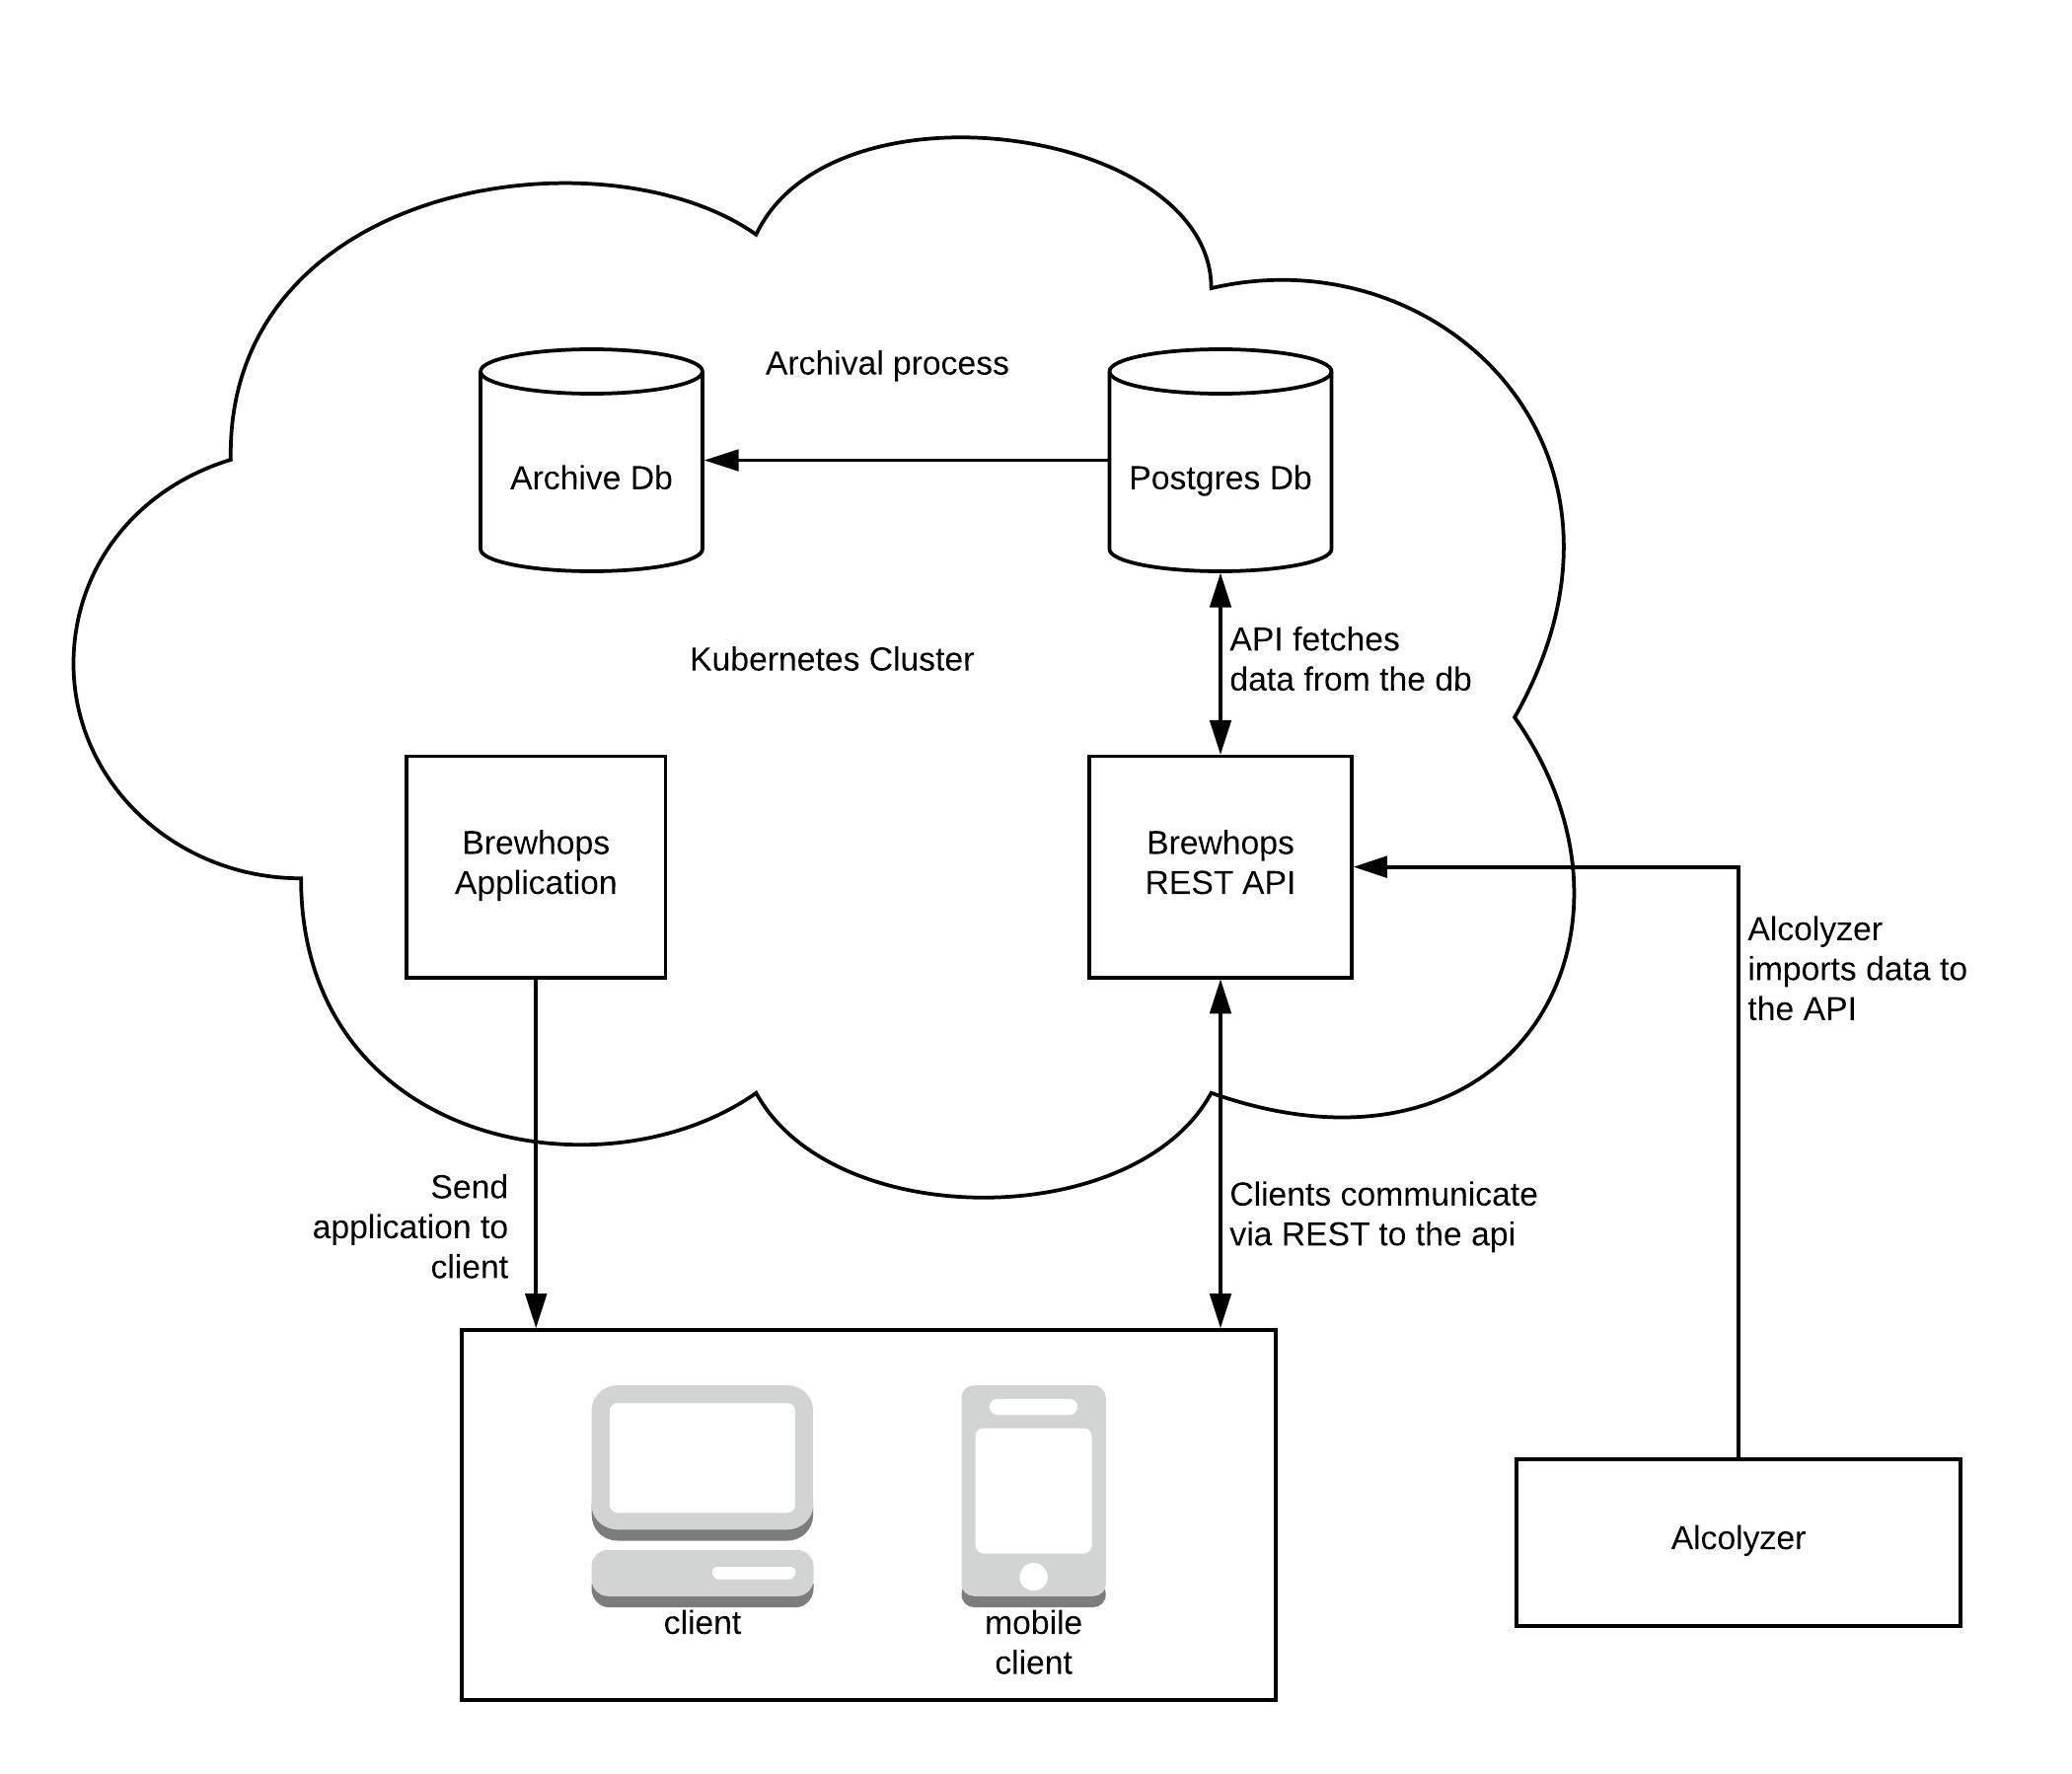
\includegraphics[origin=c,width=\textwidth,keepaspectratio]{./diagrams/brewhops-architecture.jpeg}
    \label{System Architecture}
\end{figure}

The BrewHops system is designed with microservice architecture, a variant of the service-based architecture. The three main software components, front-end, API, and database, are loosely coupled and do not rely on each other to run. Individual teammates will be able to develop and scale these pieces without fear of effecting other work.

The front-end is only responsible for asking the API for data and displaying it. If the data needs to change the front-end will pass that work onto the API. The API is the liaison between the front-end and database. It can create, read, update and delete data from the database. The database itself is only responsible for storage. The BrewHops team has experience designing microservice systems from industry. The reason that the team has chosen this pattern is because of its compatibility with cloud hosting services and simplicity rather than combined team experience. 
\section{Design}

    \subsection{Database}
    
    This section lays out the design of the database.  It includes all changes that need to be made to the current schema to account for the software requirements that have been laid out.
    
        \subsubsection{Existing}
        The existing database already has the core entities that are needed to keep track of all of the required information.  The different batches of beer, their version measurements, recipes, and tanks (the containers that the batches are brewed in) all already exist.  Different entities for providing a rudimentary task system also exist, these include: Tasks, Actions, and Employees.  The employee entity also represents the user object with user name and password fields.  The layout of the database can be seen in the ER diagram at figure \ref{erd}.
        
        \begin{figure}
            \centering
            \caption{ER diagram for the existing database schema.}
            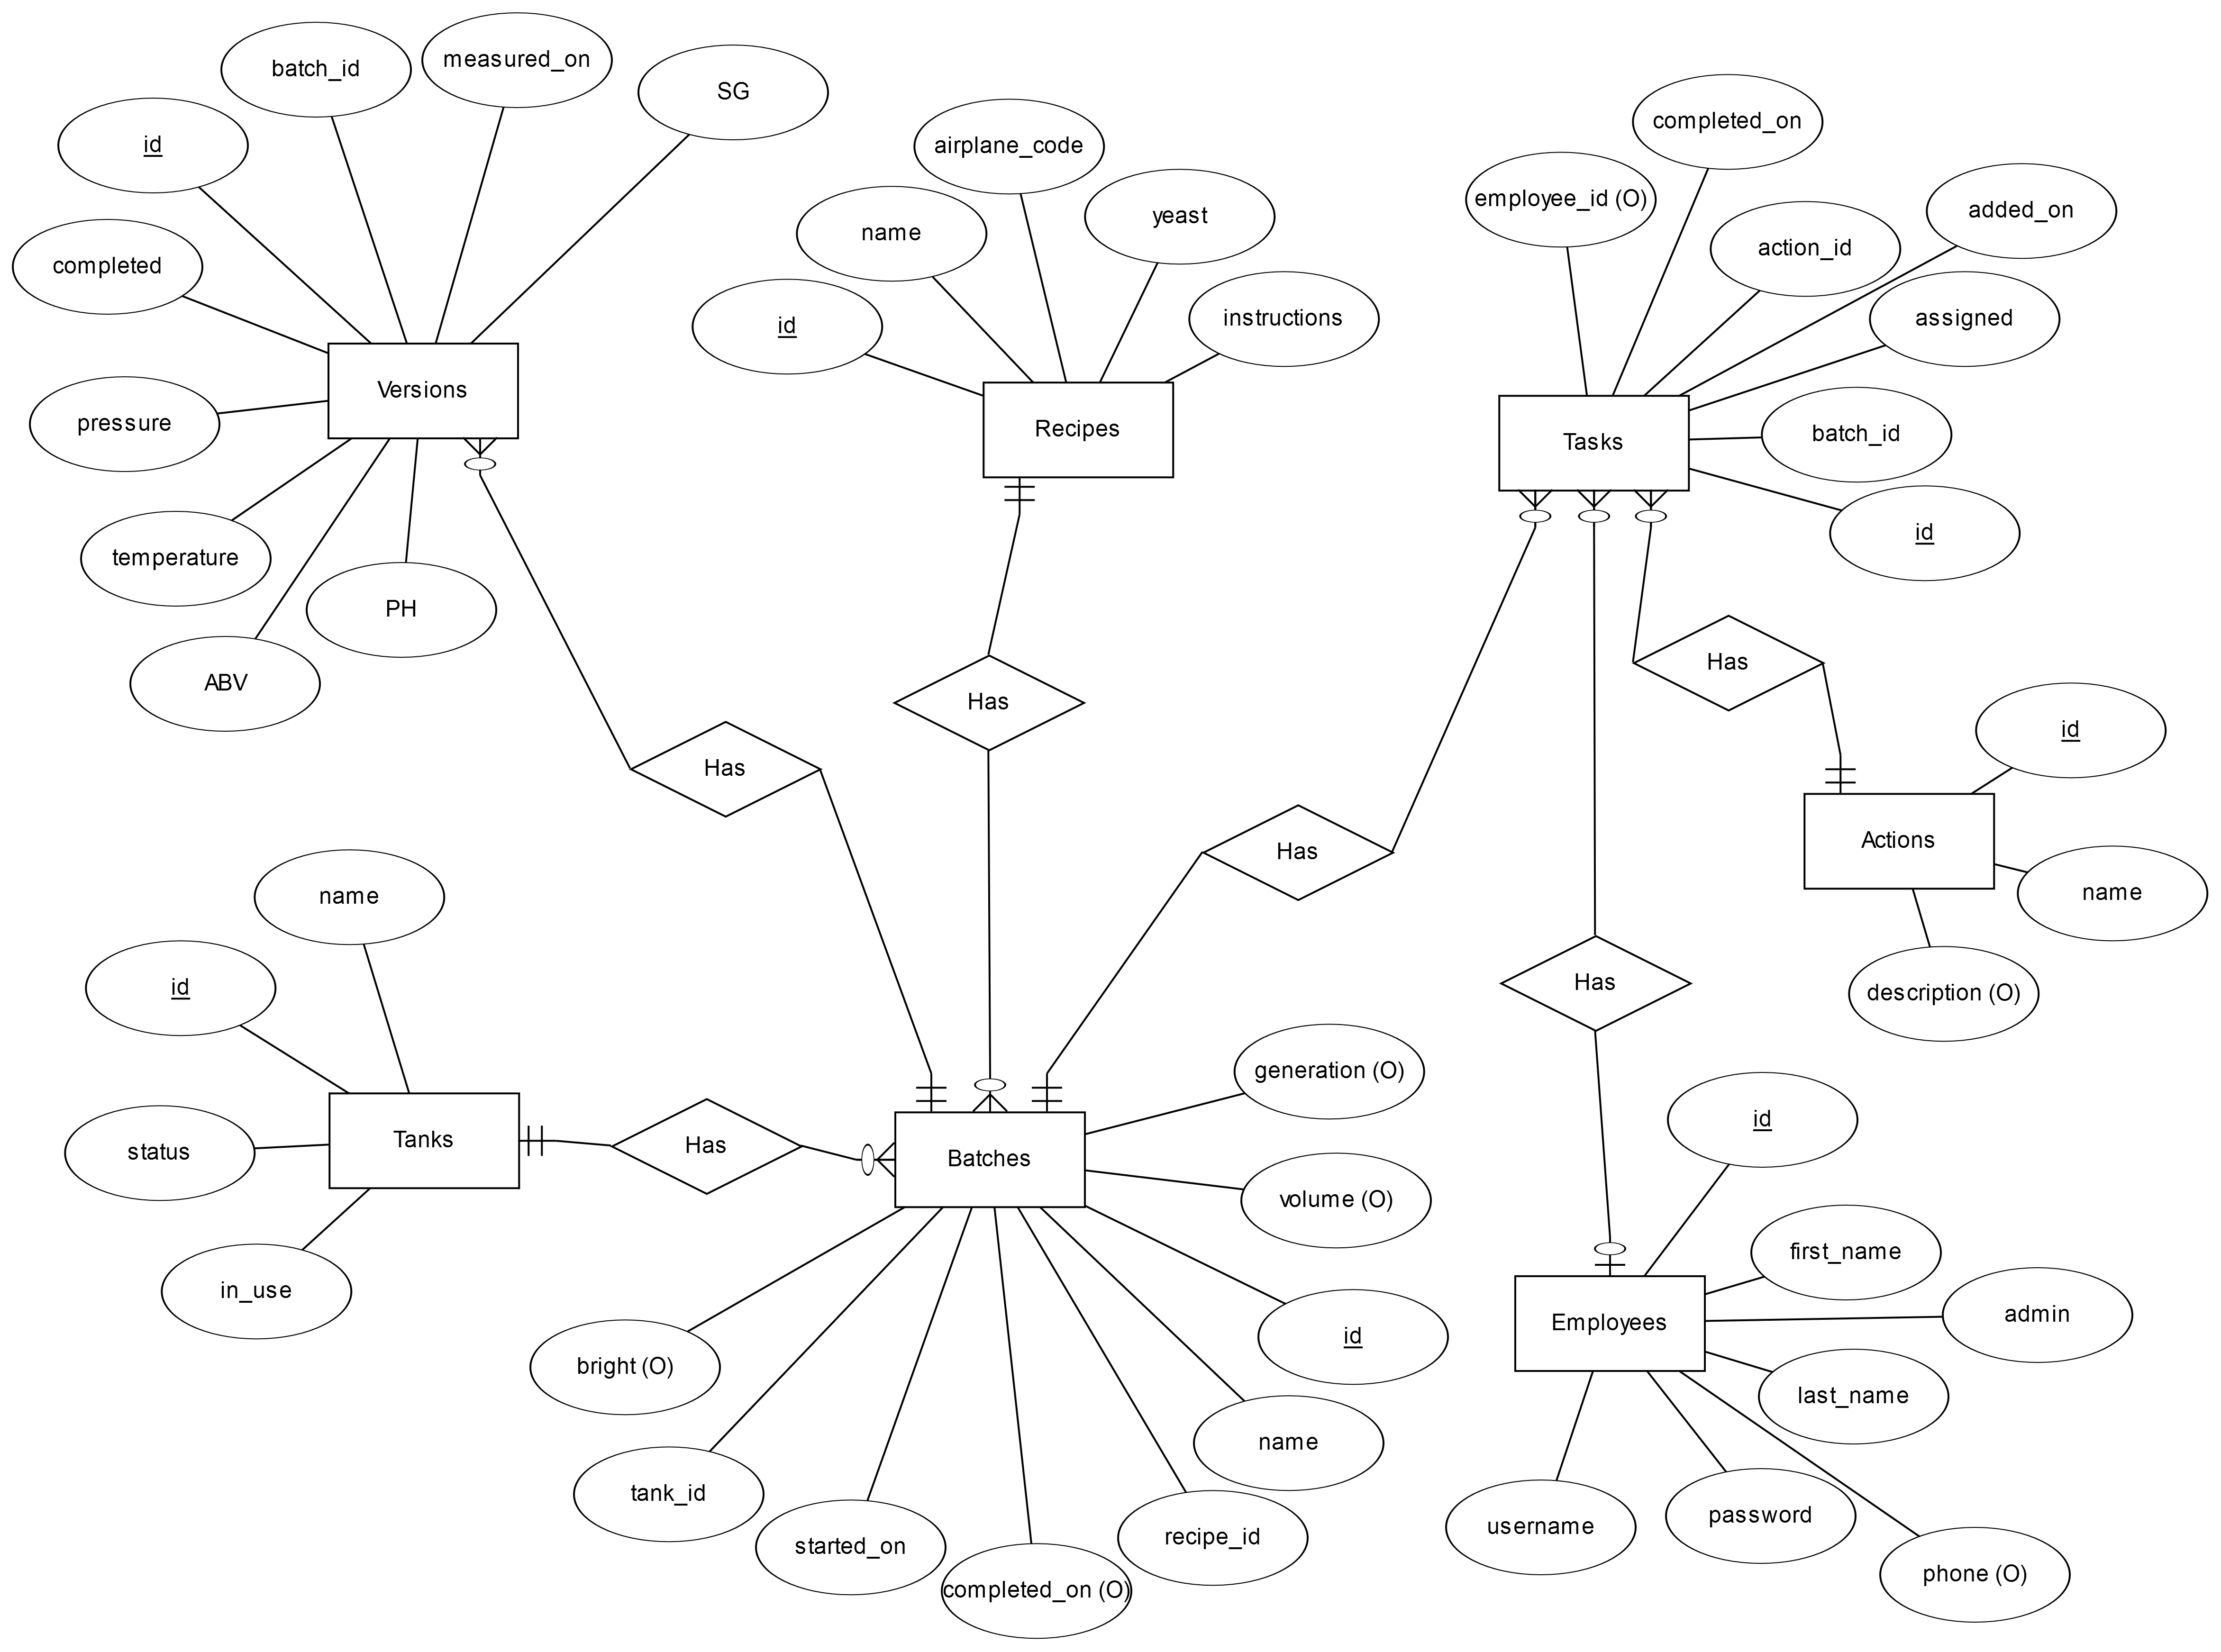
\includegraphics[angle=90,origin=c,width=\textwidth,keepaspectratio]{./diagrams/erdplus-diagram.png}
            \label{erd}
        \end{figure}
    
        \subsubsection{Updates}
        First, security needs to be updated.  Plain text passwords shouldn't be kept in the database as it is major security vulnerability. To resolve this, the password attribute on Employee will be converted into a password hash.  Upon log in, the given password can be hashed again and compared against the stored hash.  This still allows the user to log in but no longer stores their password in plain text.
        
        Next, new functionality defined by the requirements document requires some additions.  Every edit that is made to one of the tables needs to be tracked so that they can be audited.  The person who made the changes also needs to be tracked.  To accomplish this auditing every table will have a "last\_updated\_by" column added to it which will hold the id of the Employee entity who last updated that row.  The edits will then be kept track of by implementing "shadow" tables for each entity.  A shadow table is a table that is exactly identical to the table schema it is "shadowing".  The shadow table makes a new row every time a change occurs to its counter part.  The action associated with this change is tracked (e.g. insert, update, and deletes) and the previous/updated values are stored in the new row (which contains a reference to the row that was changed).  These shadow tables' naming schema will match the name of their respective table with "\_history" appended onto it.  These shadow tables will be implemented with trigger on each of the possible actions: insert, update, delete.
        
        An example of an updated table definition with a shadow table is:\\
        
        \begin{minted}[
            xleftmargin=18pt,
            linenos,
            autogobble,
            breaklines,
        ]{sql}
            CREATE TABLE IF NOT EXISTS recipes (
                id              SERIAL      NOT NULL PRIMARY KEY,
                name            VARCHAR(30) NOT NULL,
                airplane_code   VARCHAR(50) NOT NULL,
                yeast           INT         NULL,
                instructions    JSONB       NOT NULL,
                last_updated_by SERIAL      NOT NULL
            );
            
            CREATE TABLE IF NOT EXISTS recipes_history (
                id              INT         NOT NULL PRIMARY KEY,
                recipe_id       SERIAL      NOT NULL,
                name            VARCHAR(30) NOT NULL,
                airplane_code   VARCHAR(50) NOT NULL,
                yeast           INT         NULL,
                instructions    JSONB       NOT NULL,
                last_updated_by SERIAL      NOT NULL
            );
        \end{minted} 
    
        Here a new column was added to the recipe table, "last\_updated\_by" that will hold the id of the last employee to update the row.  Then the shadow table, "recipes\_history", was created.  The id represents the id of the shadow table and the id that represents the recipes id has been moved to "recipe\_id".  Foreign key relationships on these ids have purposely been left off as it causes issues when every table has a reference to one other one.  And there is no foreign key for the shadow table's reference to the recipe row as when the row gets deleted it will no longer exist but the shadow table should still hold the data.
    
    \subsection{Front-end}
    \subsubsection{View}
    The front-end application will aim to be as light as possible and rely on the external API rather that its own server to authenticate users and access data. It will be written in Vue.js, taking advantage of the single file component (SFC) pattern. An SFC file contains three sections: the view template, logic, and styling. This is contrary to traditional web design where those three sections, namely HTML, CSS, and JavaScript, were largely separated into their own files. 

    The app will be a single page application (SPA) that will simply switch out SFCs when the user navigates to different pages. The main page component will render its sub-components, also SFCs, preserving separation of concerns. Data and functionality will flow through the application from the top down, as shown in figure 3. This means that any data a component needs to render itself will be passed through by its parent. Additionally, if the parent needs to perform some action based on its child component, a function is passed to the child that it can call to notify its parent.
    
    \subsubsection{Communication}
    A client interface will be defined to encapsulate the logic for communication with the API. With TypeScript we can define the types that will be returned by the interface, apply static type-checking to it, and by extension to the whole application. The static type-checking will greatly decrease the development time of the front-end and eliminate time spent tracking down data-based bugs. All error handling will be taken care of inside the interface, so view logic remains simple.
    
    \begin{figure}[H]
        \centering
        \caption{Example of the data flow through view components}
        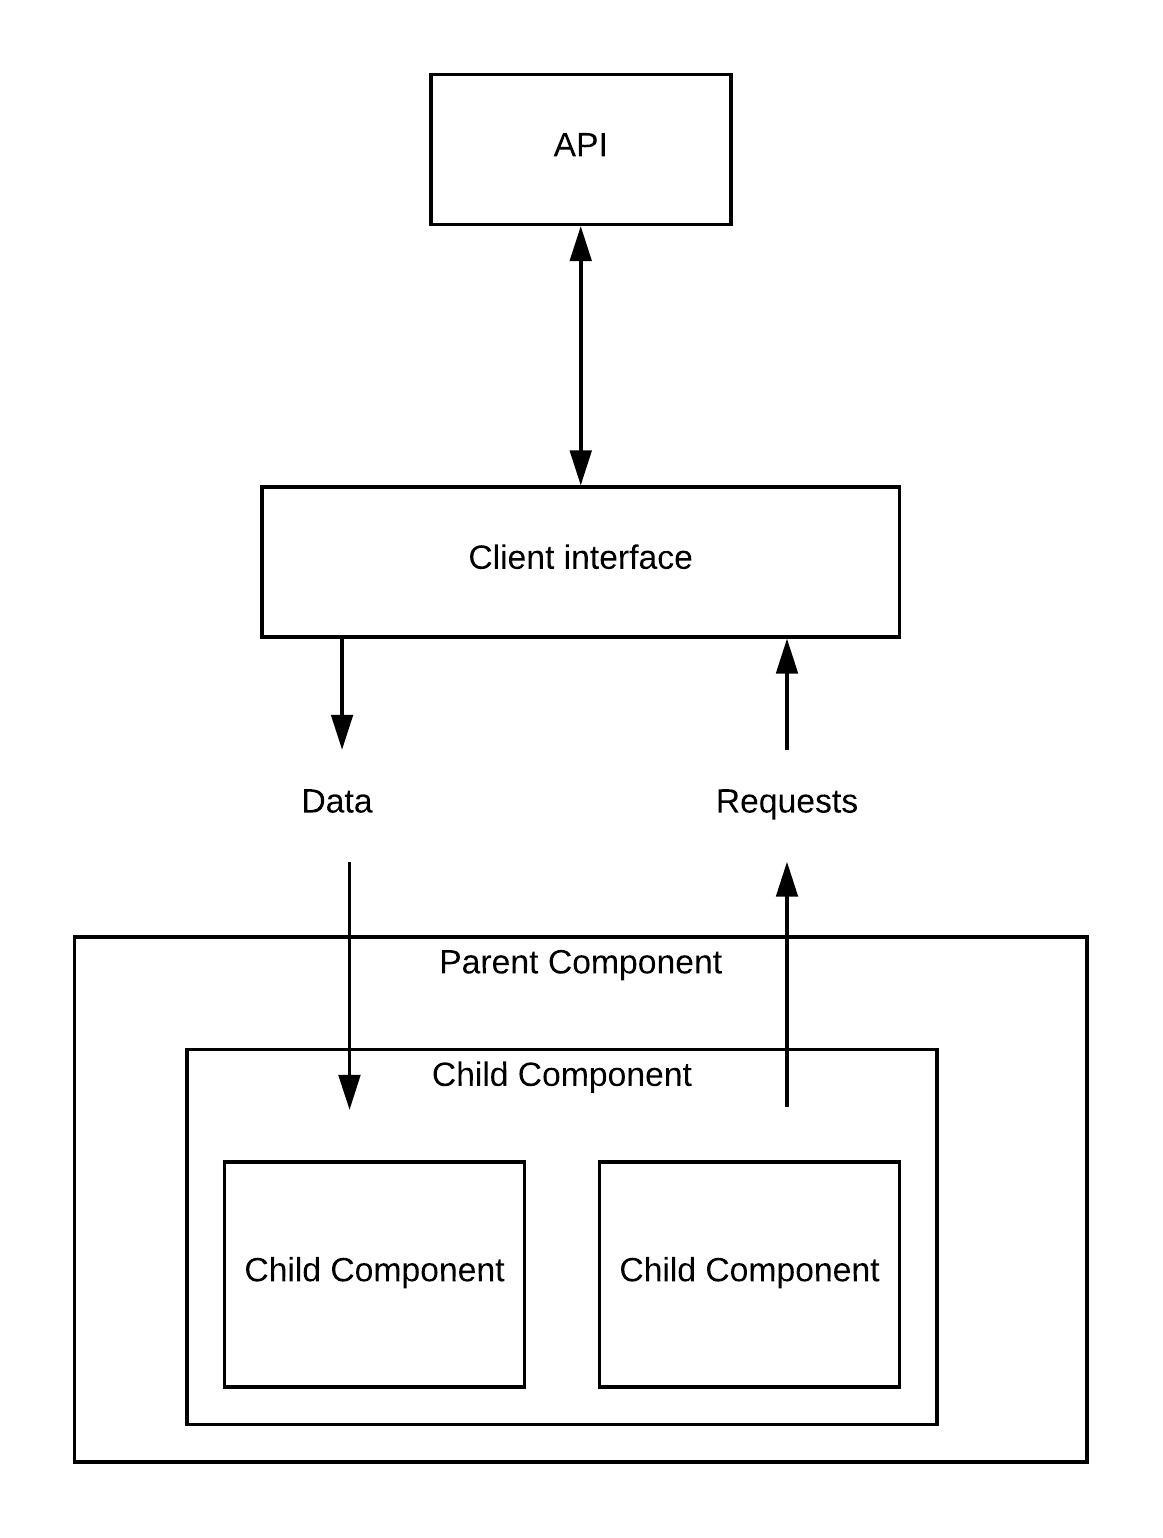
\includegraphics[origin=c]{./diagrams/front-end-diagram.jpeg}
        \label{front-end}
    \end{figure}
    
    \subsubsection{Testing}
    Testing the front-end app is a relatively new trend in web development and it has been made very easy with libraries like Jest, written by Facebook. Jest can send mocked data through the app and take “snapshots” of the rendered components. When front-end code changes, the tests will fail in an expected way, then the developer can confirm the changes made with the new snapshot. When tests fail unexpectedly, this is still good, because Jest is catching some unwanted side effects that need to be addressed.

    In addition to snapshot testing, functional testing is available to test any visual dynamic behavior. For example, if there is a drop-down menu, a good unit test for it would be that it opens and closed accordingly when clicked. Although it is tedious test for a human to do, Jest allows us to automate it, so the team benefits from additional unit testing without spending the extra time on it.
    
    \subsection{API}
    \subsubsection{Typescript Conversion}
    We will convert the back-end code from pure Javascript to Typescript because it is a super-set of JavaScript and therefore backwards compatible. The process of converting will be fairly quick. This will primarily involve defining types and adding those types to the appropriate variable declarations and functions. Types provide better readability for those coming to the project as well as ensure robustness in code as it is written. The following is an example of a JavaScript function compared with its TypeScript counterpart.\\
    JavaScript:
    \begin{minted}[
        xleftmargin=18pt,
        linenos,
        autogobble,
        breaklines,
    ]{javascript}
        buildUpdateString (keys, values) {
            keys = keys.split(',')
            let query = ``
            let idx = 1
            for (var i in keys) {
              let key = keys[i]
              query += `${key} = \$${idx}, `
              idx++
            }
            query = query.substring(0, query.length - 2)
            return {
              query,
              idx
            }
          }
    \end{minted}
    TypeScript:
    \begin{minted}[
        xleftmargin=18pt,
        linenos,
        autogobble,
        breaklines,
    ]{javascript}
        buildUpdateString (keys: string, values: string): IUpdateString {
            let key_list:string[] = keys.split(',')
            let query: string = ``
            let idx: number = 1
            for (let key in key_list) {
              query += `${key} = \$${idx}, `
              idx++
            }
            query = query.substring(0, query.length - 2)
            return {
              query,
              idx
            }
          }
        \end{minted}
        In the situation above, the type \verb:IUpdateString: would also have to be defined, but it would also be used in other functions that return the same type of value.
    \subsubsection{New Functionality}
        Due to updates being made in the database and the front-end, we will have to similarly update the back-end so that data can be passed between the two without issue. This functionality will mirror much of the logic already implemented and will be written directly in TypeScript. It will have query functions to update and retrieve data from new database tables as well as REST protocol functions to update the user interface and receive changes.
    \subsubsection{Testing}
        We will write testing for the back-end using Jest. This requires that we create a mock database for these functions to hit, running different types of valid and invalid data through them. We will make sure that all types of valid data presents us with correct results and that invalid data is handled properly such that it does not crash the application. This will improve the consistency of the application by showing that at least all of the known cases can be handled. It will also help with future development because team members can check that, when they make changes, the application still behaves in the expected fashion.
        
    \subsection{Dev-Ops}
        \subsubsection{Container}
            Docker will be used as our container for each instance of our application. The Docker containers will allow us to compartmentalize instances, giving us the ability to test and deploy multiple in a very short amount of time. It will help considerably if the website gets heavy traffic, preventing it from being bogged down with many requests. This will be the first part of the Dev-Ops tasks that will need to be setup as this is the most basic building block of our web application.
             
            These containers will be set up on virtual machines hosted on Amazon Web Services, which are then load balanced. Once the Docker containers are fully functional and tested, we can then move on to setting up the load balancer.
            
        \subsubsection{Cloud Storage and Load Balancing}
            We will handle load balancing and storage through Amazon Web Services.
            The containers will need to live somewhere, and so will the data they collect. Using Amazon Web Services, we will be able to spin up our containers on the cloud, and use Amazon's Elastic Load Balancing tools to direct traffic. 
            With multiple containers getting an even amount of traffic through the load balancer, we should not have a problem with constant up-time and little to no downtime on our site. 
            
            Amazon Web Services will also be where we can store our database of information on tanks, batches, history, etc. The information will be available to all of the Docker containers, and will be accessed through the client interface to the API. See \textbf{section 3.2.2} for more information on sending and receiving information to the API.
    
            Once we have load balanced Docker containers, we can test traffic throughput and make sure our load balancer can handle enough if not more traffic than we anticipate. Once we move past the load balanced container and have it all set up correctly, we can host it on Amazon Web Service's EC2.  
        
        \subsubsection{Web Hosting}
            As of now, the website is hosted on a previous student's Oregon State ENGR server. Our goal is to take the site down, and set it up on a more professional, business-grade environment.
            Similarly to our Cloud Storage and Load Balancing, we will be using Amazon's EC2 hosting option to distribute our website. Amazon's EC2 gives us a lot of easy options when working in unison with their elastic load balancer. EC2 hosting will take requests and forward them to our load balancer, which will be the elastic load balancer. From there, the load balancer will decide on which Docker Container the user should go to, based on traffic.
            
            Web hosting can be tested easily, using Amazon Web Services built-in diagnostic tool, and also by checking the container id's when going through each instance. It can be usability tested also by checking and seeing if the sites load properly. 
            
        \begin{figure}[h]
            \centering
            \label{fig:my_label}
            \caption{Left side represents our Web Hosting URL. It then cascades down to the Load Balancer and then to each instance and container}
            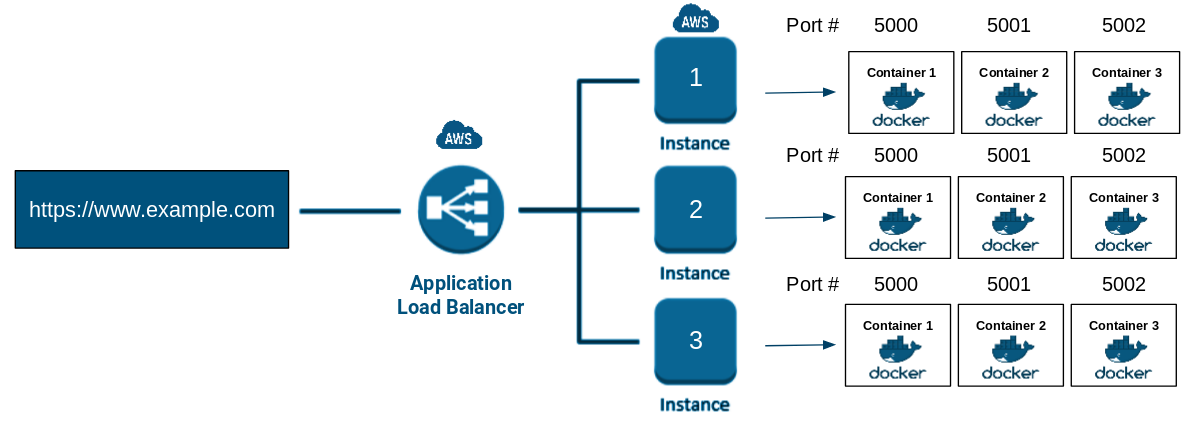
\includegraphics[width=6.5in]{img/load-balance-architecture.png}
        \end{figure}          
    
\section{Appendix}
    \subsection{Desktop Design}
    \begin{figure}[H]
        \centering
        \caption{The Login page for desktop}
        \fbox{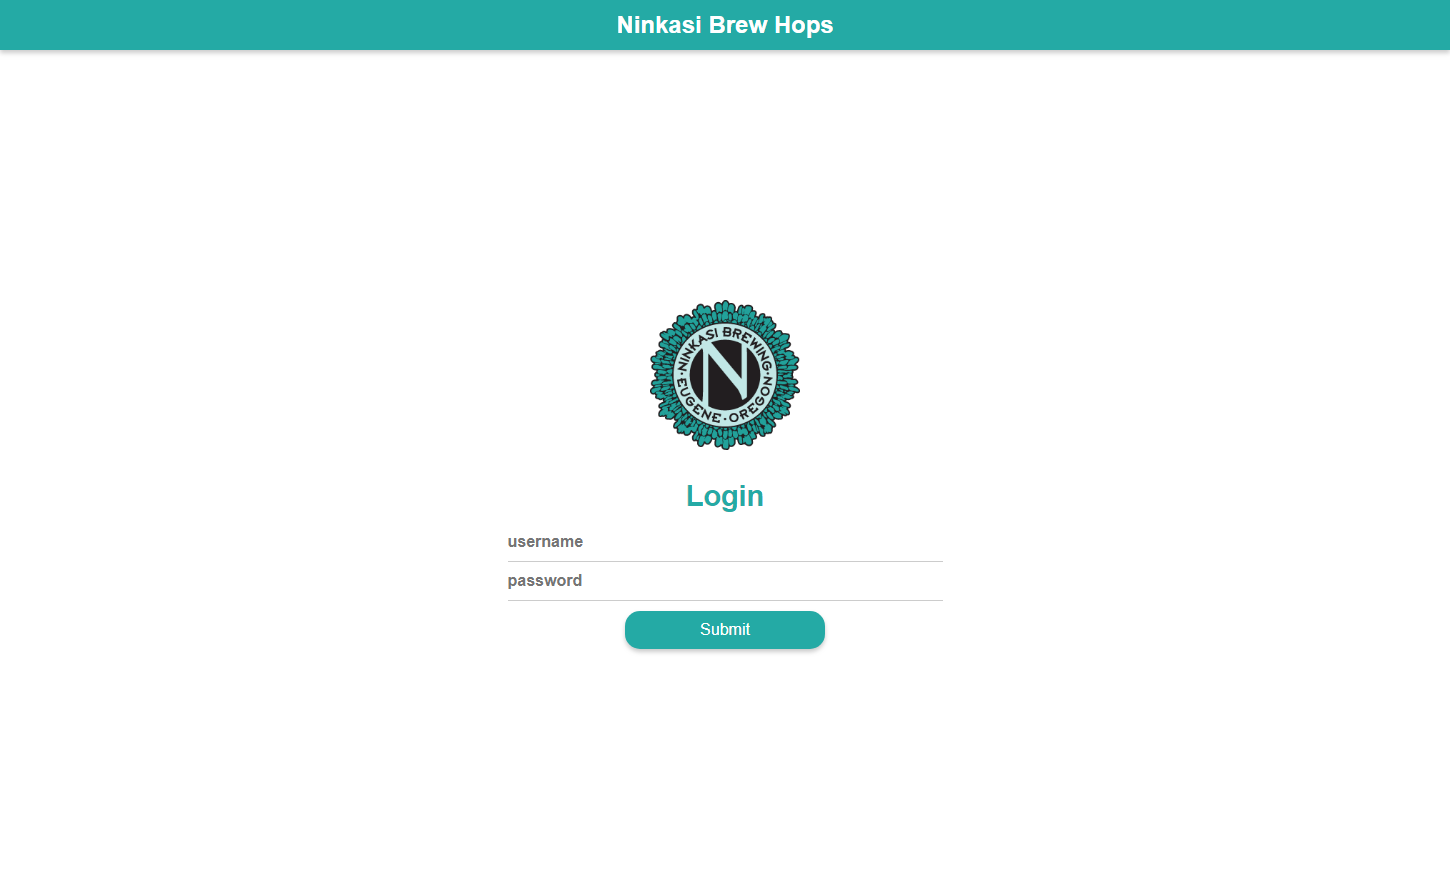
\includegraphics[origin=c,width=6in,keepaspectratio]{./img/login-page.png}}
        \label{login-page}
    \end{figure}
    \begin{figure}[H]
        \centering
        \caption{The desktop homepage}
        \fbox{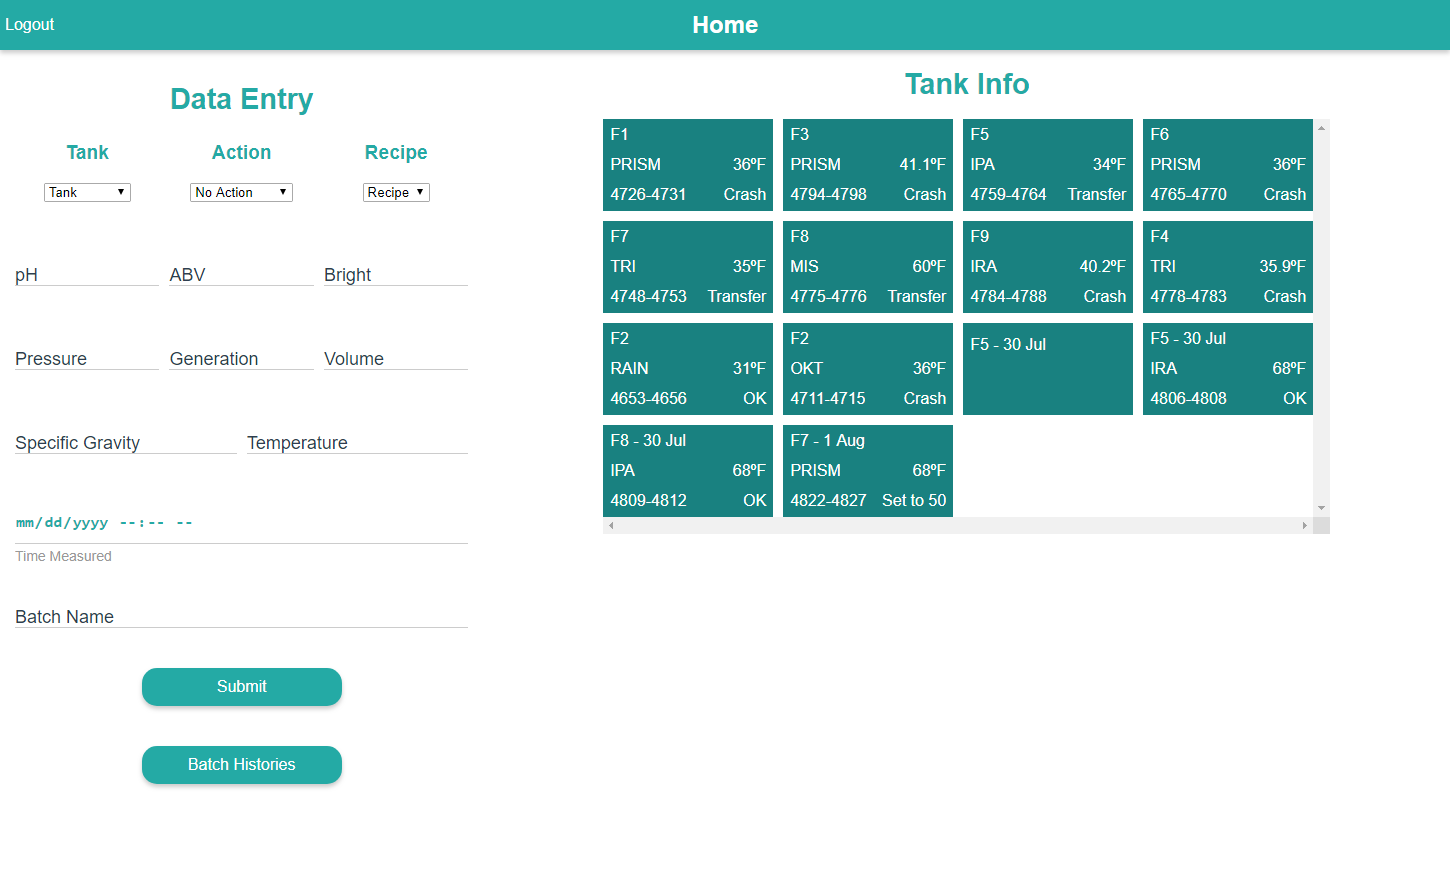
\includegraphics[origin=c,width=6in,keepaspectratio]{./img/home-page.png}}
        \label{home-page}
    \end{figure}
    \begin{figure}[H]
        \centering
        \caption{The tank information page}
        \fbox{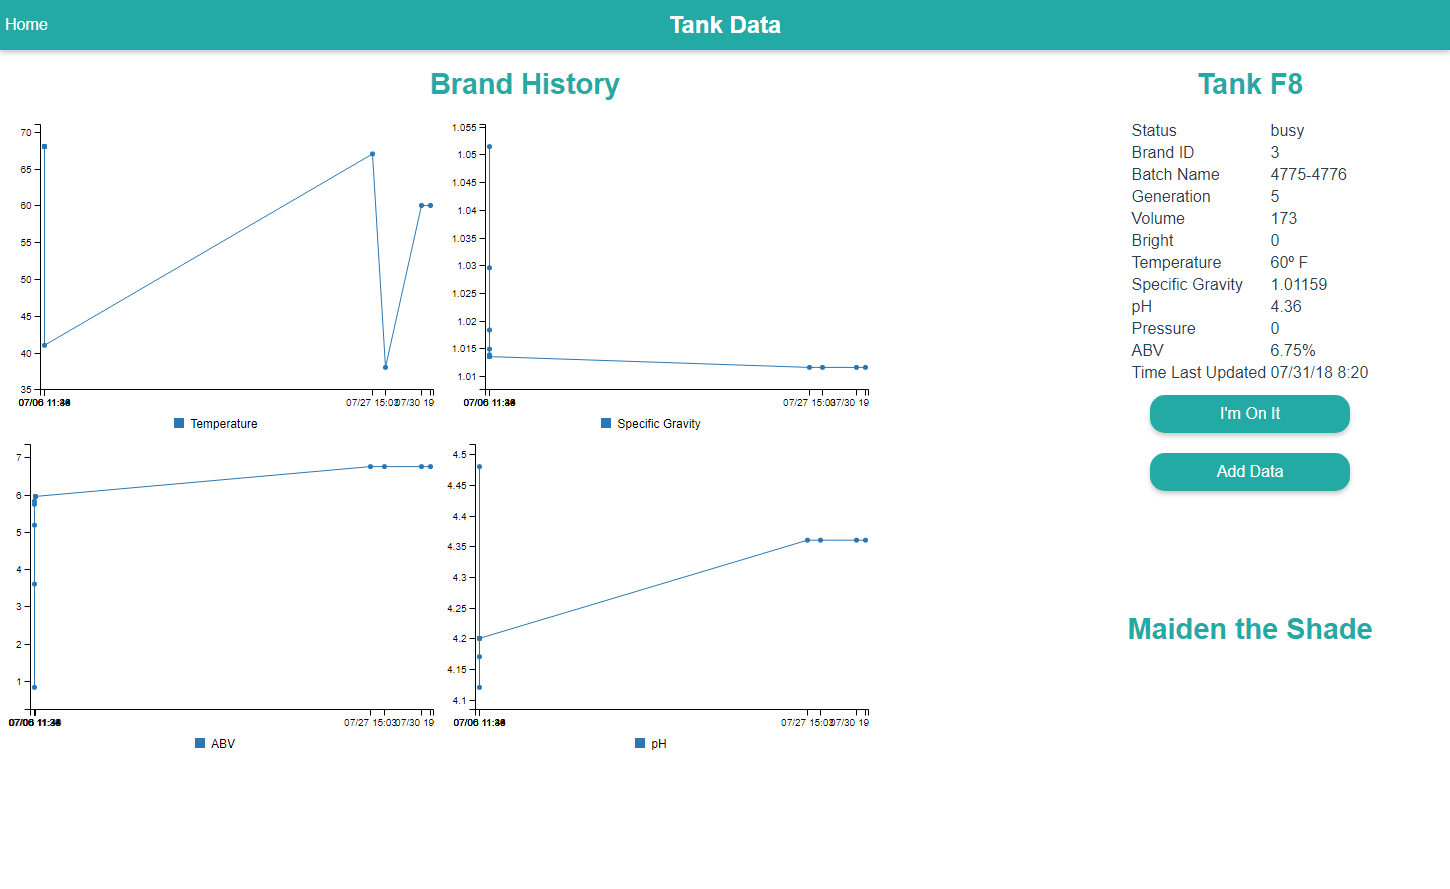
\includegraphics[origin=c,width=6in,keepaspectratio]{./img/tank-page.png}}
        \label{tank-page}
    \end{figure}
    \begin{figure}[H]
        \centering
        \caption{The data entry page}
        \fbox{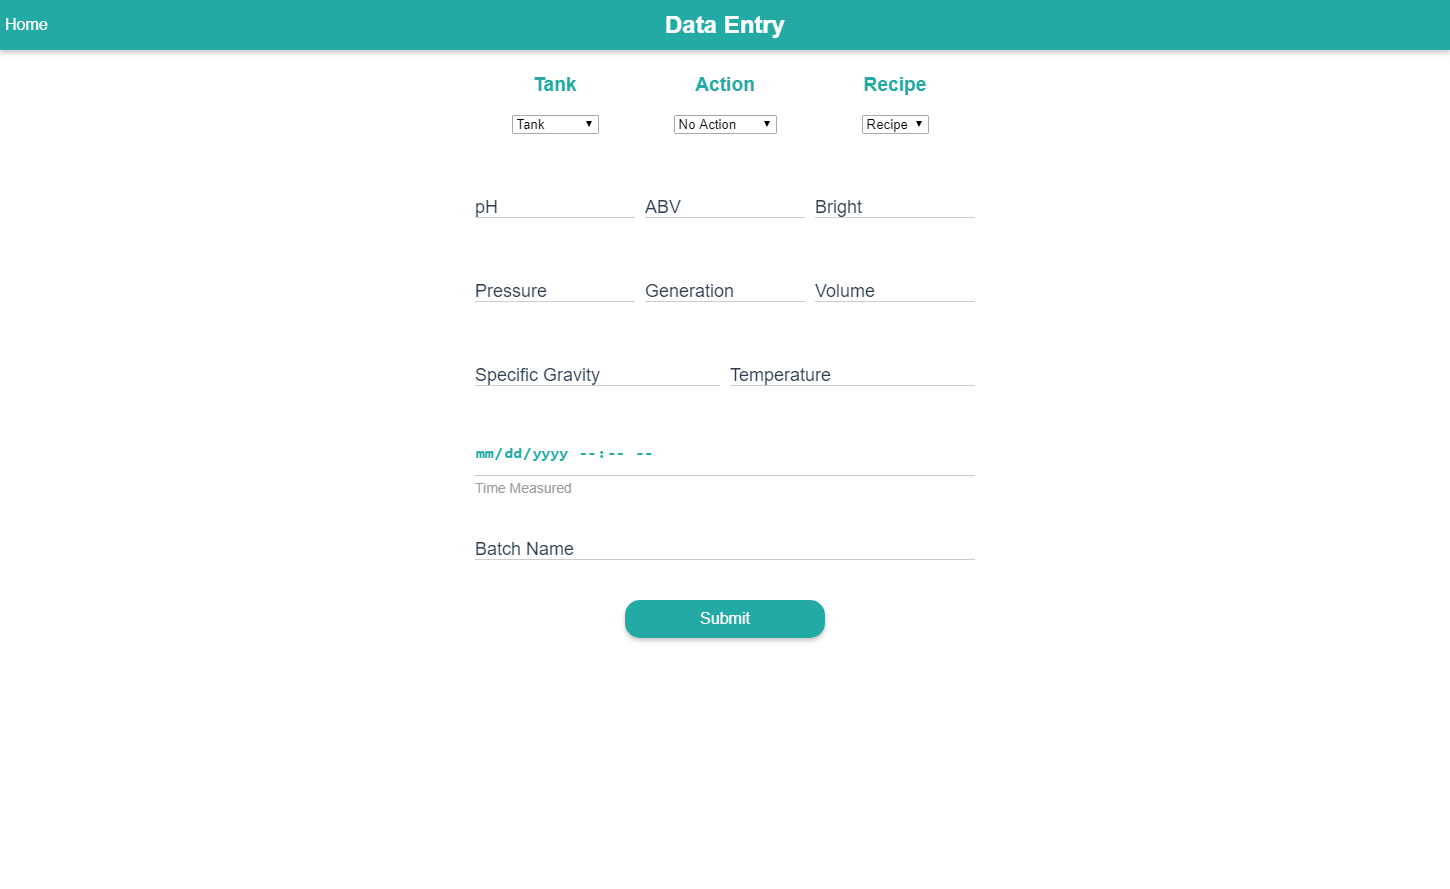
\includegraphics[origin=c,width=6in,keepaspectratio]{./img/data-entry.png}}
        \label{data-page}
    \end{figure}
    
    \subsection{Mobile Design}
    \begin{minipage}[t]{0.3\textwidth}
    \sidesubfloat{
        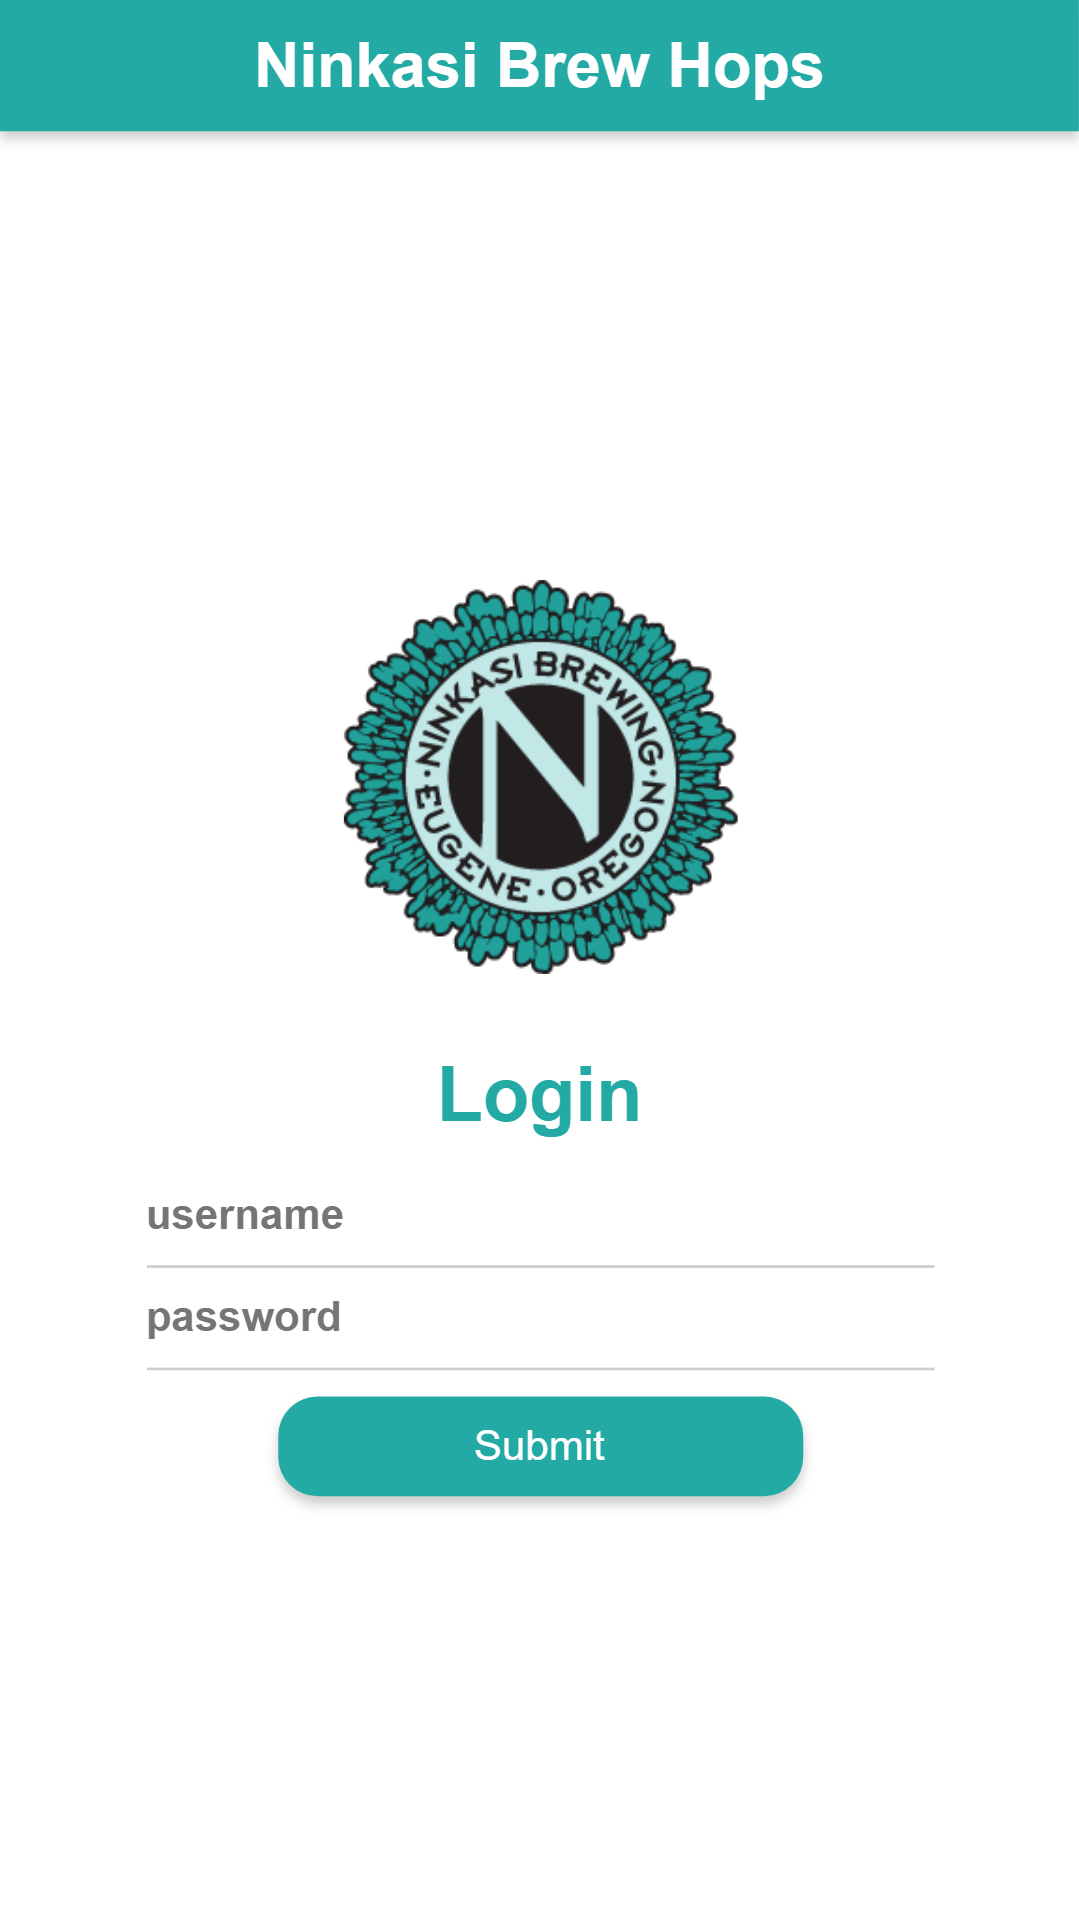
\includegraphics[width=\textwidth]{./img/mobile-login-page.png}
        \caption{Mobile login page}
        \label{fig:mobile-login-page}}
    \end{minipage}
    \begin{minipage}[t]{0.3\textwidth}
    \sidesubfloat{
        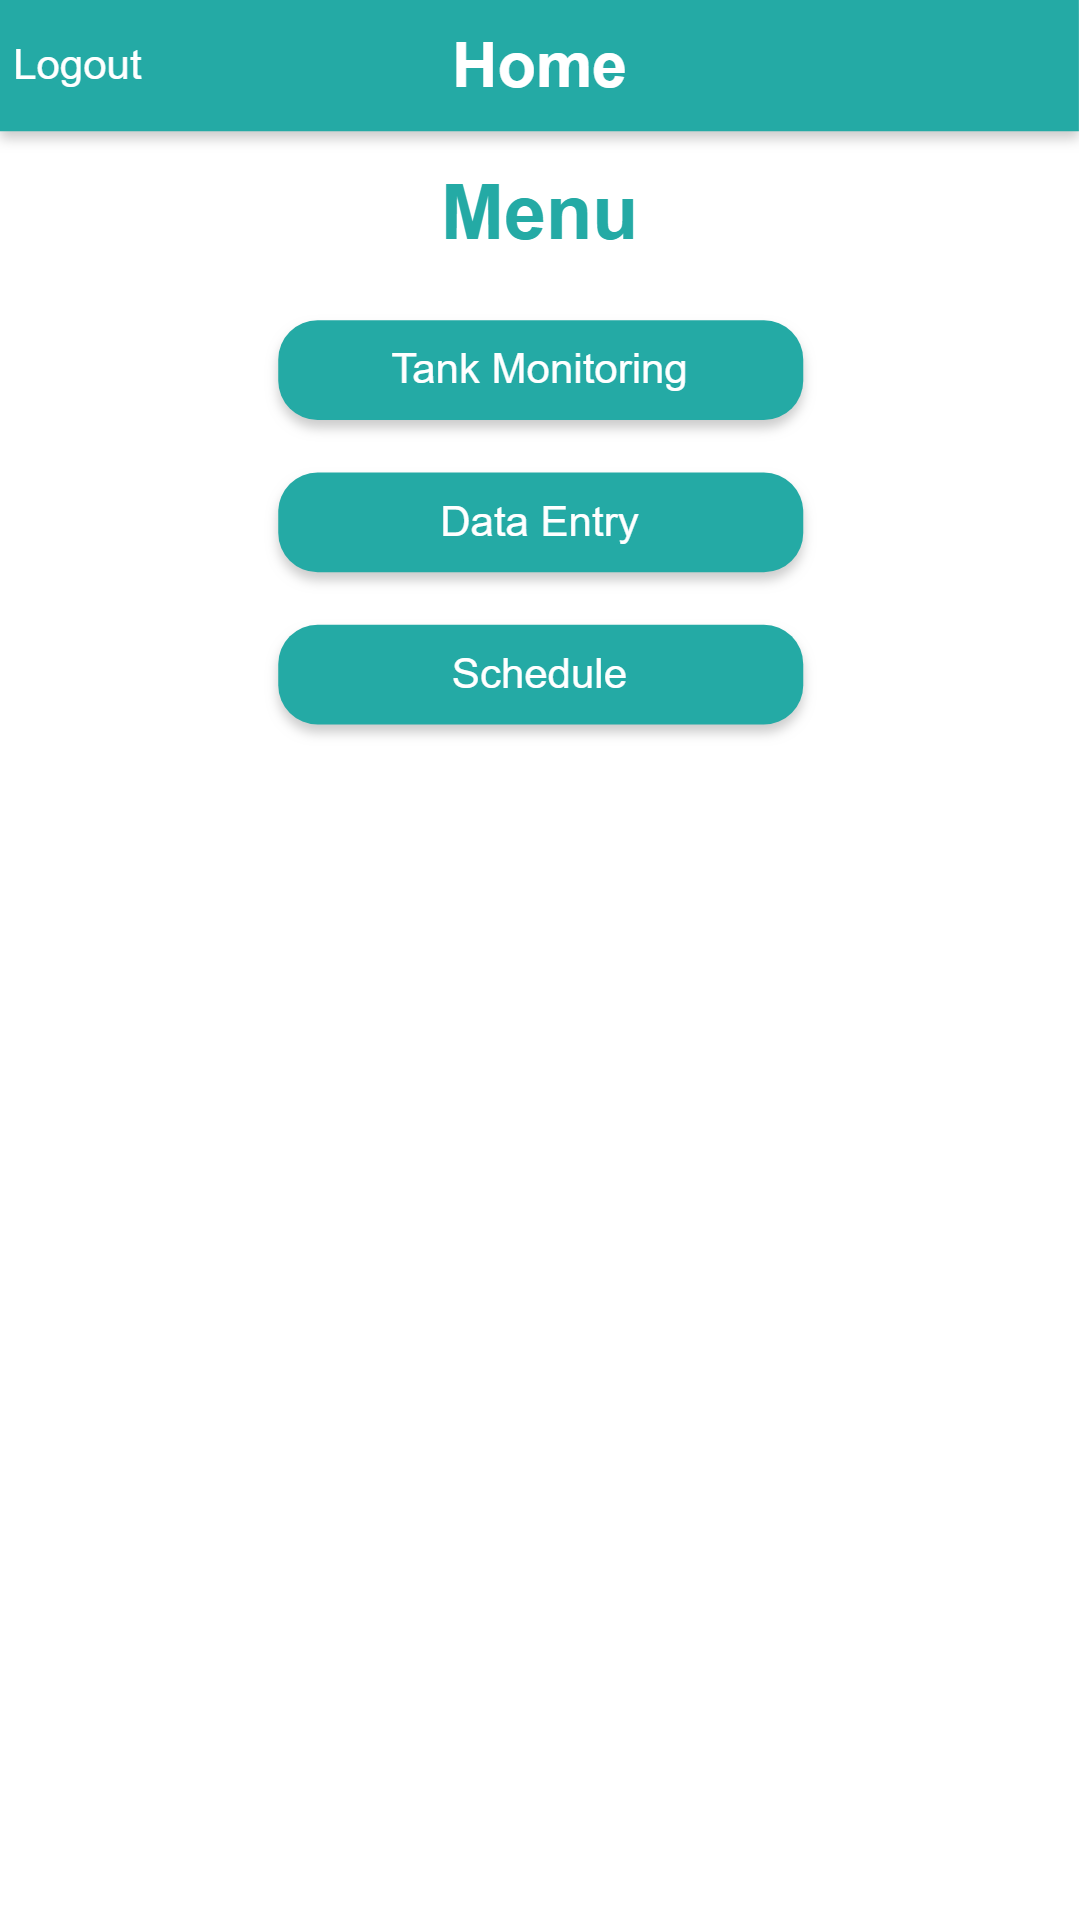
\includegraphics[width=\textwidth]{./img/mobile-home-page.png}
        \caption{Mobile home page}
        \label{fig:mobile-home-page}}
    \end{minipage}
    \begin{minipage}[t]{0.3\textwidth}
    \sidesubfloat{
        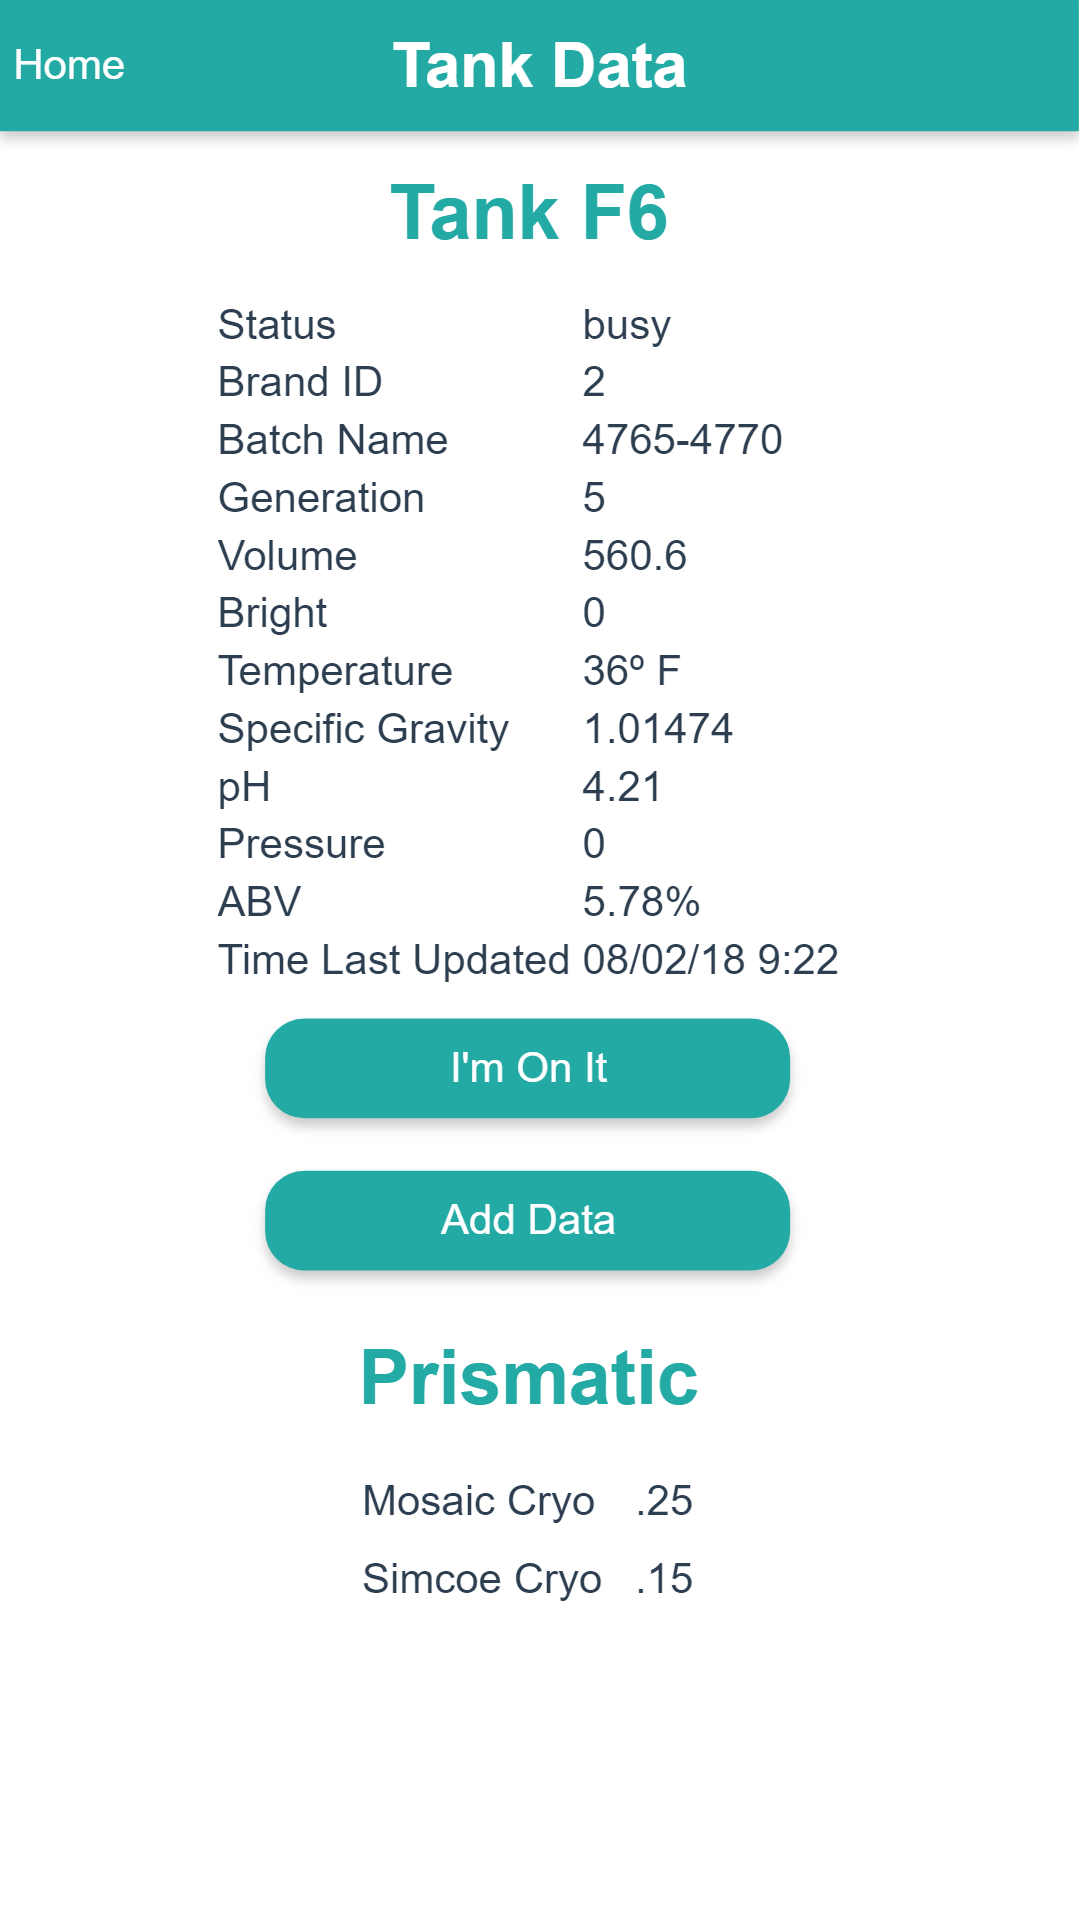
\includegraphics[width=\textwidth]{./img/mobile-tank-page.png}
        \caption{Mobile tank page}
        \label{fig:mobile-tank-page}}
    \end{minipage}
    
    \begin{minipage}[t]{0.3\textwidth}
    \sidesubfloat{
        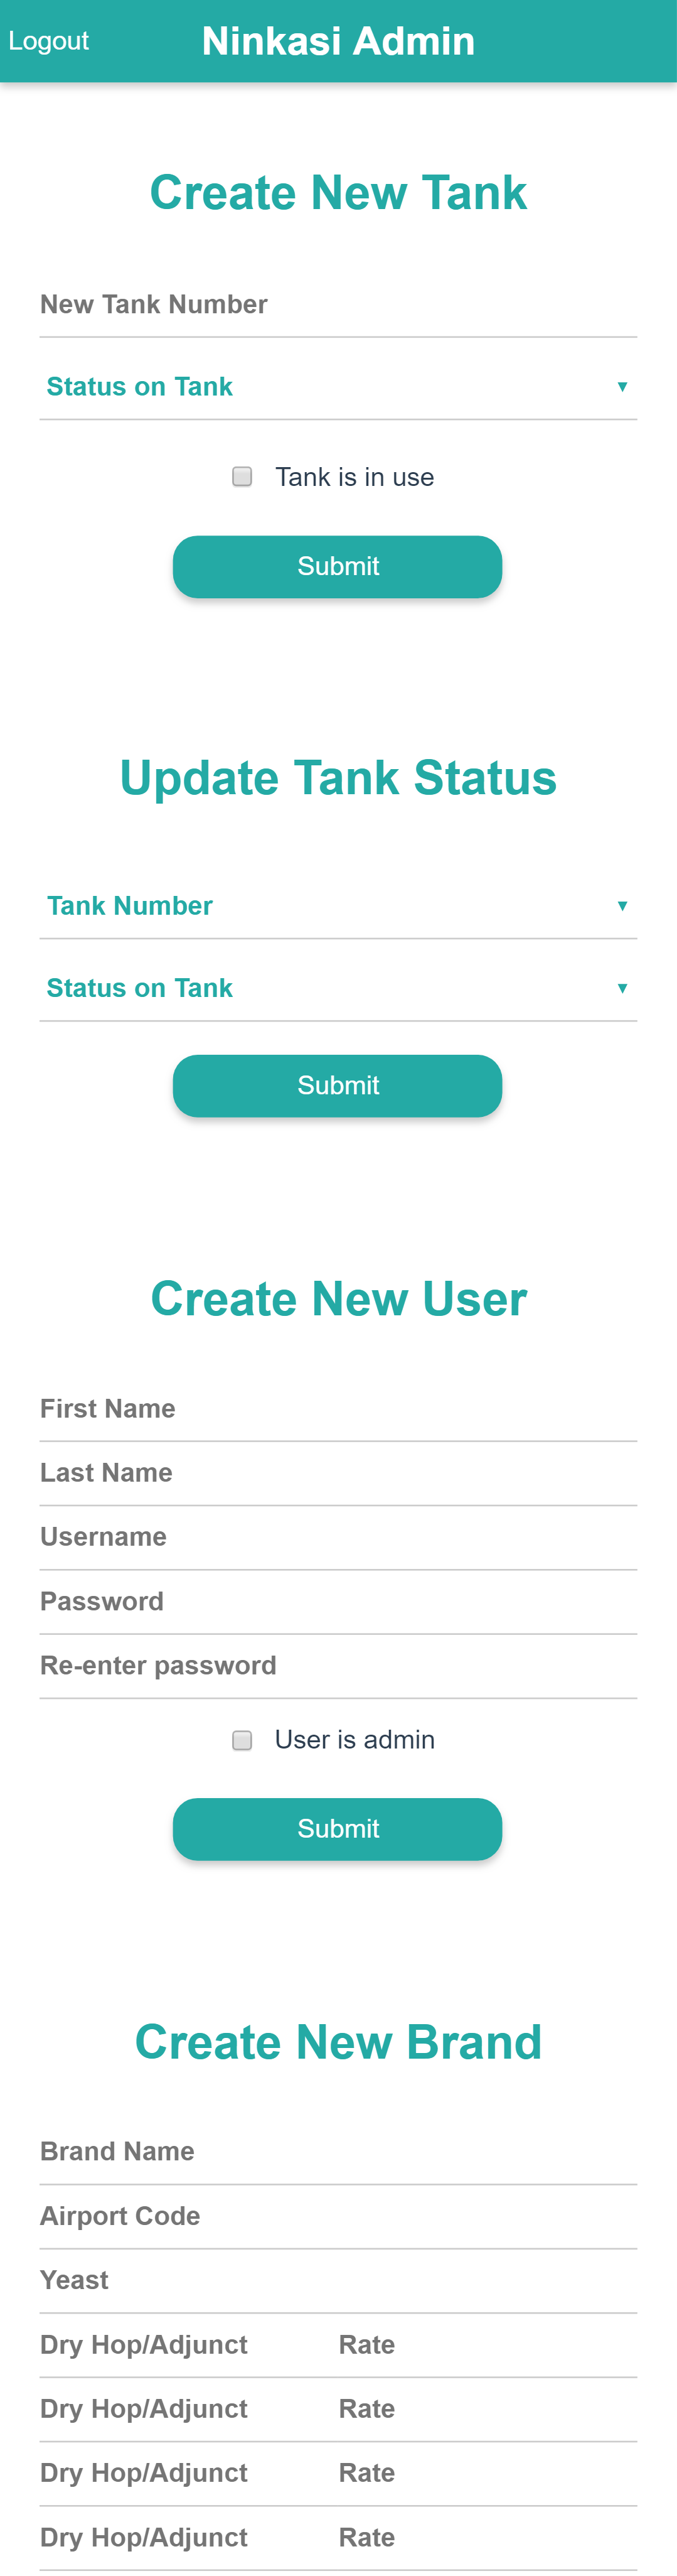
\includegraphics[width=5cm,align=t,keepaspectratio]{./img/mobile-admin-page.png}
        \caption{Mobile admin page}
        \label{fig:mobile-login-page}}
    \end{minipage}
    \begin{minipage}[t]{0.3\textwidth}
    \sidesubfloat{
        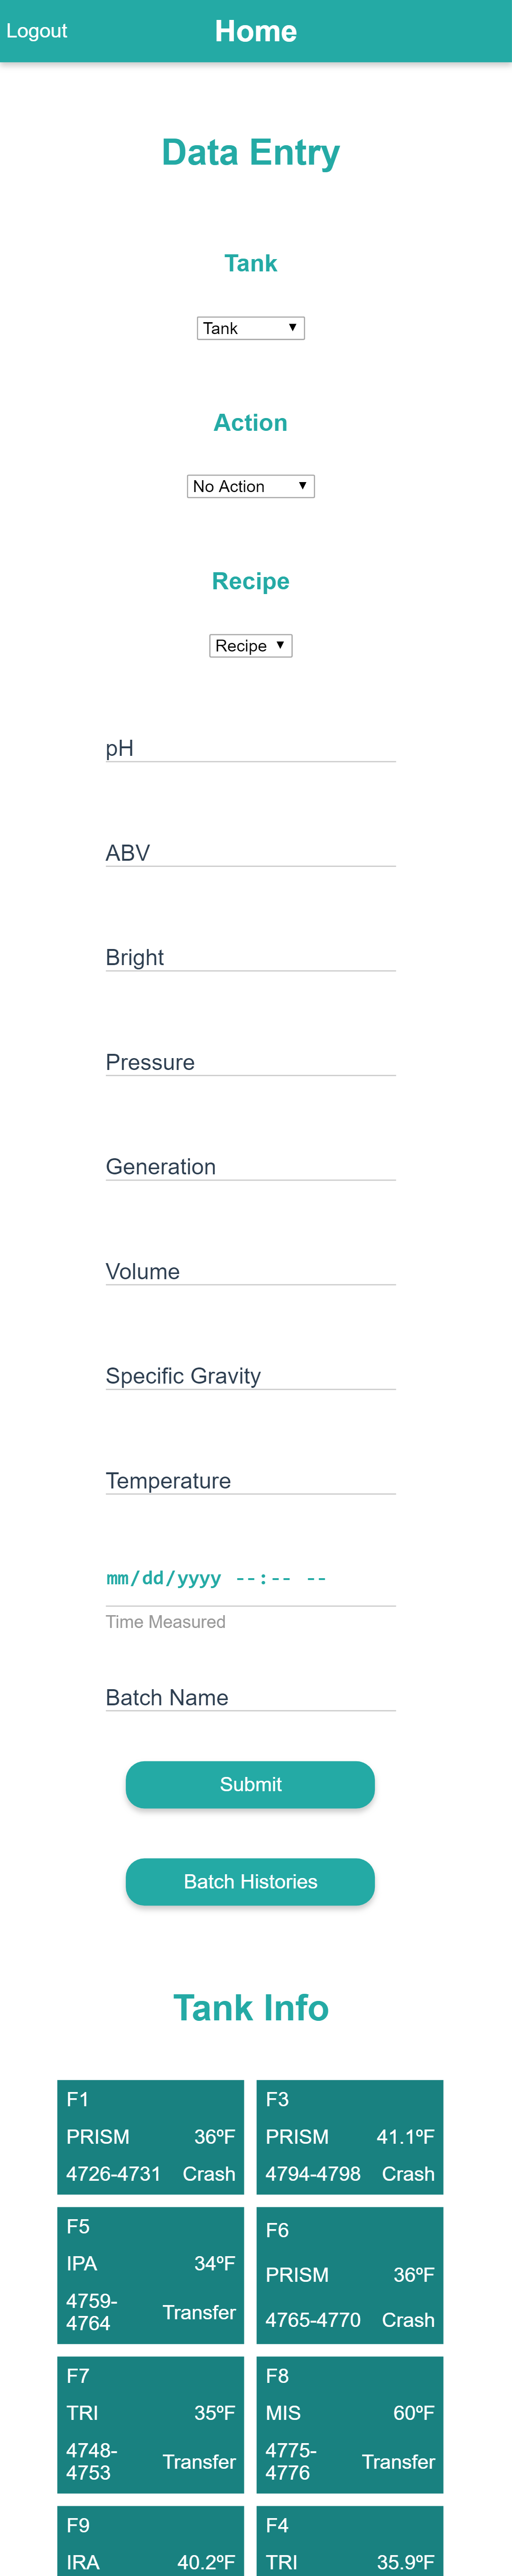
\includegraphics[width=5cm,align=t,keepaspectratio]{./img/mobile-data-entry.png}
        \caption{Mobile data entry page}
        \label{fig:mobile-data-entry-page}}
    \end{minipage}
    \begin{minipage}[t]{0.3\textwidth}
    \sidesubfloat{
        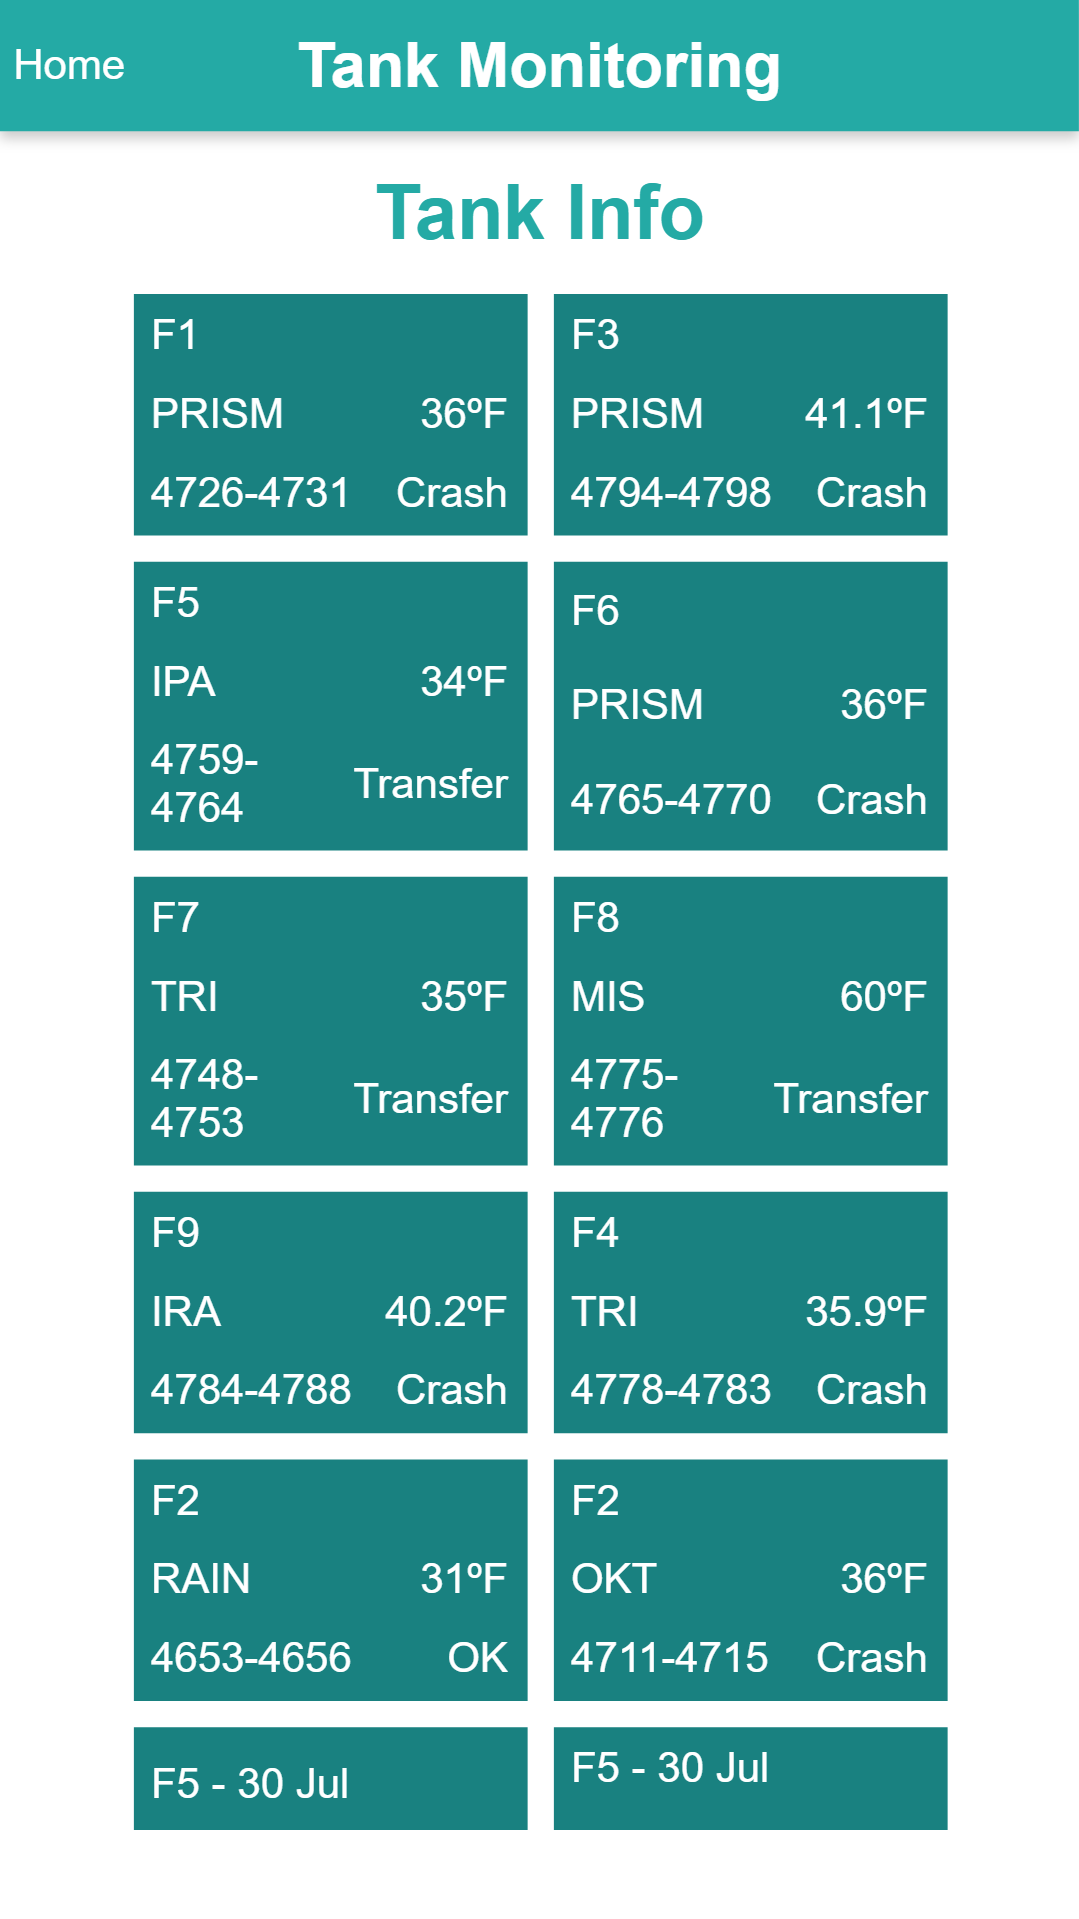
\includegraphics[width=5cm,align=t,keepaspectratio]{./img/mobile-tank-info-page.png}
        \caption{Mobile tank info page}
        \label{fig:mobile-tank-info-page}}
    \end{minipage}

\bibliographystyle{IEEEtran}
\bibliography{./ref}

\end{document}
